% !TEX root = ../thesis.tex
% !TEX spellcheck = en-US

%% In a thesis, every section starts a new page, hence \clearpage
\clearpage

\section{Exploration}
\label{sec:Exploration}

The first part of this thesis project was dedicated to exploration of the problem space. Driven by the research objectives the goal was twofold: At once to find an approachable yet challenging research problem in the context of data from a recruitment platform while simultaneously evaluating the potential for creating value through an enhanced user experience or new use cases for the service.

\subsection{Discovery Phase: Exploring the Problem Scope}
\label{Discovery Phase: Exploring the Problem Scope}

During the discovery phase the problem space was first opened up through exploration of user needs and initial field research better understand the problem context. Additionally literature research and benchmarking of approaches helped getting a picture of related scientific work. It should be noted though that quantitative user research was rather minimal due to time constraints and the scientific nature of this thesis.

Initially a set of early interviews with stakeholders from Product Management to Marketing and Engineering and as well potential users helped getting a good idea about the service offerings of a recruitment platform and the current trends in the industry. Exploring the various data that the platform generates the first learning was that large parts of the data are in form of written language and much of it in a more or less unstructured way.

Exploration was therefore focused on language related problems. Literature research revealed a strong interest from the research community in tasks related language modeling using neural networks and other connectionist approaches that had gained traction through the latest advances of \gls{Deep Learning}. Several methods were then tested as quick prototypes, also leading to the learning that real data is often noisy and inconsistent. In addition ideas for focusing the problem search were evaluated, ranging from practical ideas such as predicting trends in the job marking to wilder ones such as digitalizing the complete Sanoma archive to analyze how written language evolves over time in order to predict when a text was written or to identify trending terms or even writing styles.

Through further experimentation, research and discussions the problem of better utilizing the implicit knowledge in the main text body of job listings was deemed a good fit for further focus. It was both an interesting and challenging research problem and could potentially be of practical use, e.g. when identifying the requirements for a job inside this text or other applications. This decision set the course for the definition phase to begin with more a stronger focus on converging the problem space.

\subsection{Definition Phase: Framing the Problem}
\label{sub:Definition Phase: Framing the Problem}

The definition phase of the design process is characterized by explorative convergence of the problem space through iterative reframing and refinement of the problem definition that goes hand in hand with further experimentation and learning within the new scope. For this research project it is marked by three main decision points where the problem definition was reformulated. These three iterations of converging towards a problem definition are described in the next sections in terms of rationale for the chosen direction, the experimental approach and testing metrics to learn within this new scope and the results and learnings obtained.

\subsubsection{Inferring Structure of Job Advertisements}
\label{subs:Inferring Structure in Job Advertisements}

\paragraph{Rationale}
\label{par:Rationale}

During the discovery phase it became apparent that a there is large amounts of unstructured and implicit knowledge in the data of job advertisements. This knowledge is difficult to access and process in a systematic and automized way, making it hard to employ for providing increased value to users. The majority of this knowledge is given in free-form natural language, e.g. making up the text body of a job advertisement. This part --- analogous to the content of a job listing in print media --- contains all the information about a job position that a company wants to communicate to a potential applicant. \todo{example?}

Certain parts of this unstructured text are of particular interest to the company, e.g. the section describing the requirements for a job because being able to utilize this knowledge enables the service platform to potentially match users with more relevant job advertisements.
Another interesting application of machine learning to enhance the user experience is to study and potentially predict successfulness of job advertisements.
The need to understand what makes a successful job ad arrises especially for recruiters writing these ads as they might be interested to better reach the talent they need. In order to design a better algorithm to analyze the success factors if job ads it is useful to first understand the structure and content of the job ad.
It has to be noted that success in this context leaves much room for interpretation as different measures of success could be incorporated, such popularity measured by \gls{click-through rate} or \gls{page views}. Such a measure has the shortcoming of not taking into account the demographics and degree of specialization of the job and other factors that are expected to have a strong influence on the target audience.

\paragraph{Experimental Approach and Metrics}
\label{par:Experimental Approach and Metrics}

This prototype was carried out in order to understand better how humans interpret structure and content of job ads and what they consider a good structural representation of the topics and information contained. In this context of facilitating applications by better understanding and representing the structure of job advertisements a first series of experiments was designed.

Five participants from various professional background were asked to highlight sections of the text of a job ad presented to them and label these sections by describing what the section “talks about”. Afterwards they were asked to restructure the job ad into a bullet-point list based on these highlighted sections.

There were no specific metrics as this prototype was purely open to gain a basic understanding how “structure” and “content” or “topics” are interpreted.
The goal was to get a better understanding how users would structure job applications, leaving the interpretation of the verb ``structure'' completely open.

Participants were provided with a \gls{Google Docs} document given with one random job advertisement in English and the task was to first highlight parts they felt belonged to a certain part and then to structure these parts. The exact formulation was as follows:

\blockquote{Cheers for helping out with this little experiment for my thesis! My aim here is to find out how people would structure job ads to help find the relevant information faster.

You'll work with the job advertisement below. Your task is the following:
\begin{enumerate}
  \item First tag the job advertisement below into parts. Mark sections of it and use a word or two to categorize this section using the comment tool. You can tag the ad into sections however you want and even make the sections overlap. The goal here is to tag the content of the job ad that you think belongs to different categories, properties or topics. To tag the text, use the comment tool like this: ``We're looking for a Quality Buzzword Engineer.''
  \item Now fill the bullet-point list in the last section of this document with the tagged sections/categories/topics you found. It should roughly contain the same information as the ad but in a structured way using your tags. You can use sub-points categories if you want.
\end{enumerate}
In total try to spend no more than 30 minutes on this. Don't worry about it too much, the key is to just do it how it makes sense to you.}

A full example of this task as it was provided for the participants can be found in the Appendix in Section~\ref{sub:Understanding How Humans Structure Text}.

\paragraph{Results}
\label{par:Results}

Only 2 participants fully carried out the task. 2 other participants only highlighted and labelled the sections. The last participant did not even start.

All participants reported being confused about the task and after providing some helping advise by providing analogous examples (e.g. labelling the description of a car and which parts talk about the components while others talk about the owner etc.) the participants still perceived the task as very difficult as it leaves much room for interpretation.

The results quite various, especially in the following ways:

Level of abstraction: “Requirements” vs. “language requirements”
Content versus language function: “Job description section indicator” vs. “Job description”, or “Leading question”
Judgement of content quality: “Empty words”
Attribute vs. value: “Application period indicator” and “Application period”
Also some participants built a nested structure in the second part of the task while others formulated rather wide areas to group the information under.

\paragraph{Learnings and Conclusions}
\label{par:Learnings and Conclusions}

The task needs to be more clearly defined and can be split up many subtasks. Generally it was as open as identifying knowledge and structuring it in some way.

A process learning about the way the prototype was carried out is that while is was a quick way to set up an experiment and a fast way to test it was too much work and too big of a task to ask more people for. The participants were my friends and it seems improbable anyone else would spent this much time and effort for such task.


\todo{more conclusions here? check thesis blog}

\todo{objectives and learnings}

\subsubsection{Multi-label Paragraph Classification}
\label{subs:Multi-label Paragraph Classification}

With the initial results the general problem direction to infer structure of job advertisements was deemed promising and an next set up experiments was set up.

In order to classify sections of job ads by their topic in a supervised manner labelled data was needed. Therefore I built a tool so I could ask others to help me tag these sections. The tool consists of a server running a database with the chunked job ad data and a web interface for participants to tag the sections/chunks of a job ad.

\paragraph{Rationale}
\label{par:Rationale}

The goal was to produce labelled data that would be more varied (with more participants interpreting the task differently) and therefore less biased than if only I would label it. Also it was carried out leaving the task slightly open to interpretation on purpose, to understand how humans approach the task of tagging paragraphs of a job ad.

\paragraph{Implementation}
\label{par:Implementation}

\ref{sub:thesis-tagger: A Tool for Tagging Chunked Job Ads}


\paragraph{Testing Procedure and Metrics}
\label{par:Testing Procedure and Metrics}

In a first step the tool was only shown to 3 participants to see if the UI had flows and the task was understood. Based on this feedback the tool was improved (especially an example was provided) and tested with the Data Mining Research group who tagged a bunch of job ads with it. The feedback I got from there was then taken into consideration for the last iteration which then opened to the public (via social media etc.). A few days later the tool was then shared internally with Sanoma employees and set up as a competition (participants could leave their email addresses and the one with the most tagged job ads would win).

\paragraph{Results}
\label{par:Results}

The participation was a absolutely great and I received 91 tagged ads using almost 400 tags for the different sections.

\paragraph{Learnings}
\label{par:Learnings}

The main learning was that instructions must be really simple and that it helps a lot to test this in a few rounds before releasing such tool to the public. The second learning was that the competition really helped to collect a lot of data.


\todo{Picture of software setup?}

To collect first data a tool was build, consisting of a Node.js\footnote{[\ldots] Node.js is an open-source, cross-platform runtime environment for developing server-side Web applications. \url{https://nodejs.org/}} server using MongoDB\footnote{\textquote{MongoDB is a free and open-source cross-platform document-oriented database [\ldots].} Source: \url{https://en.wikipedia.org/wiki/Node.js}, Website: \url{https://www.mongodb.com}} as a database and communicating via a JSON with a simple website front-end using the mustache template engine\footnote{\textquote{Mustache is a simple web template system.} Source: \url{https://en.wikipedia.org/wiki/Mustache_(template_system)}, Website: \url{https://mustache.github.io}}.
The tool is online\footnote{\url{http://thesis.cwestrup.de/jobad-tagger/}} and it's source code is publicly available on GitHub\footnote{\url{https://github.com/cle-ment/thesis-tagger}} with it's API documentation hosted online as well\footnote{\url{http://thesis.cwestrup.de/jobad-tagger/apidoc/}}.

The data generated by using the free-form text description of each job ad and splitting it into paragraphs as can be seen in the software package as well\footnote{\url{https://github.com/cle-ment/thesis-tagger/blob/master/pre-processing.ipynb}}.

The goal of this prototype tool for data collection was on the one hand to acquire data in order to carry our first experiments as fast as possible, and on the other hand to gain a deeper understanding about the research problem itself by giving an open, unbiased task to the participants. In particular the question at hand was how humans label the content of the different parts of a job ad.

The exact task given to the participants was ``Describe what each section is about by adding one or more tags/keywords to it''. They were shown a job ad that was split into paragraphs and besides each paragraph was a text field to enter 1 or more tags.

\begin{figure}[h]
  \centering
  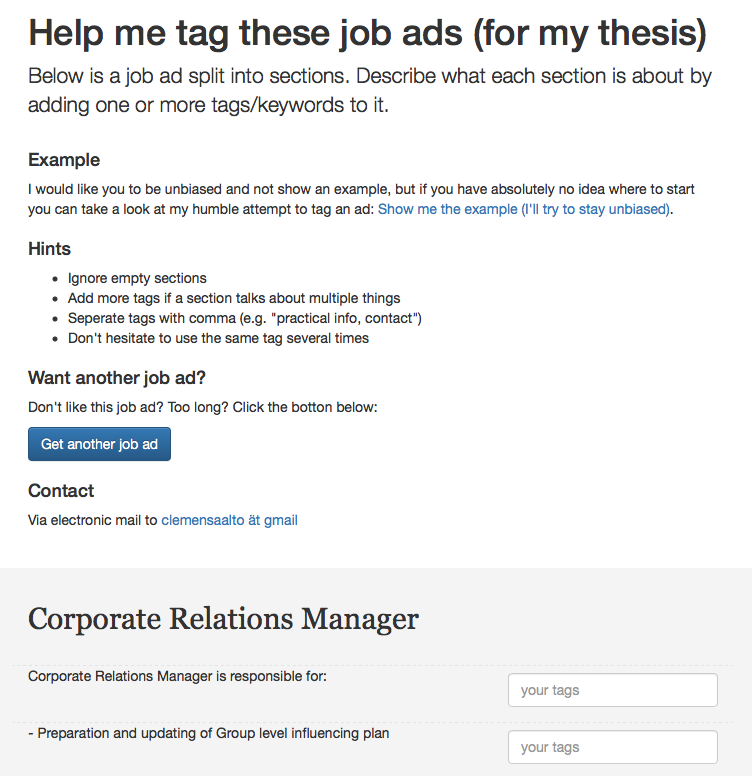
\includegraphics[width=\textwidth]{img/thesis-tagger-interface.png}
  \caption{Screen capture of the interface of the tagging tool}
\label{fig:thesis-tagger-interface}
\end{figure}

In a first step the tool was only shown to 3 participants to get immediate feedback if the user interface had flaws and whether the task was understood.   Based on this feedback the tool was improved by providing an example for the participants and then tested with a slightly larger group of 12 persons. After correcting a few minor details in the user interface a public link was then shared via social media and other channels with as many people as possible. A few days later the tool was then also shared internally within Sanoma where it was set up as a competition to tag the most possible job ads.

In total 91 job ads were tagged, resulting in 379 tagged text sections and 358 tags.

\todo{Describe data: Different characteristics}
\todo{show distribution?}
\todo{show embedding visualizations}

\begin{figure}[h]
    \centering
    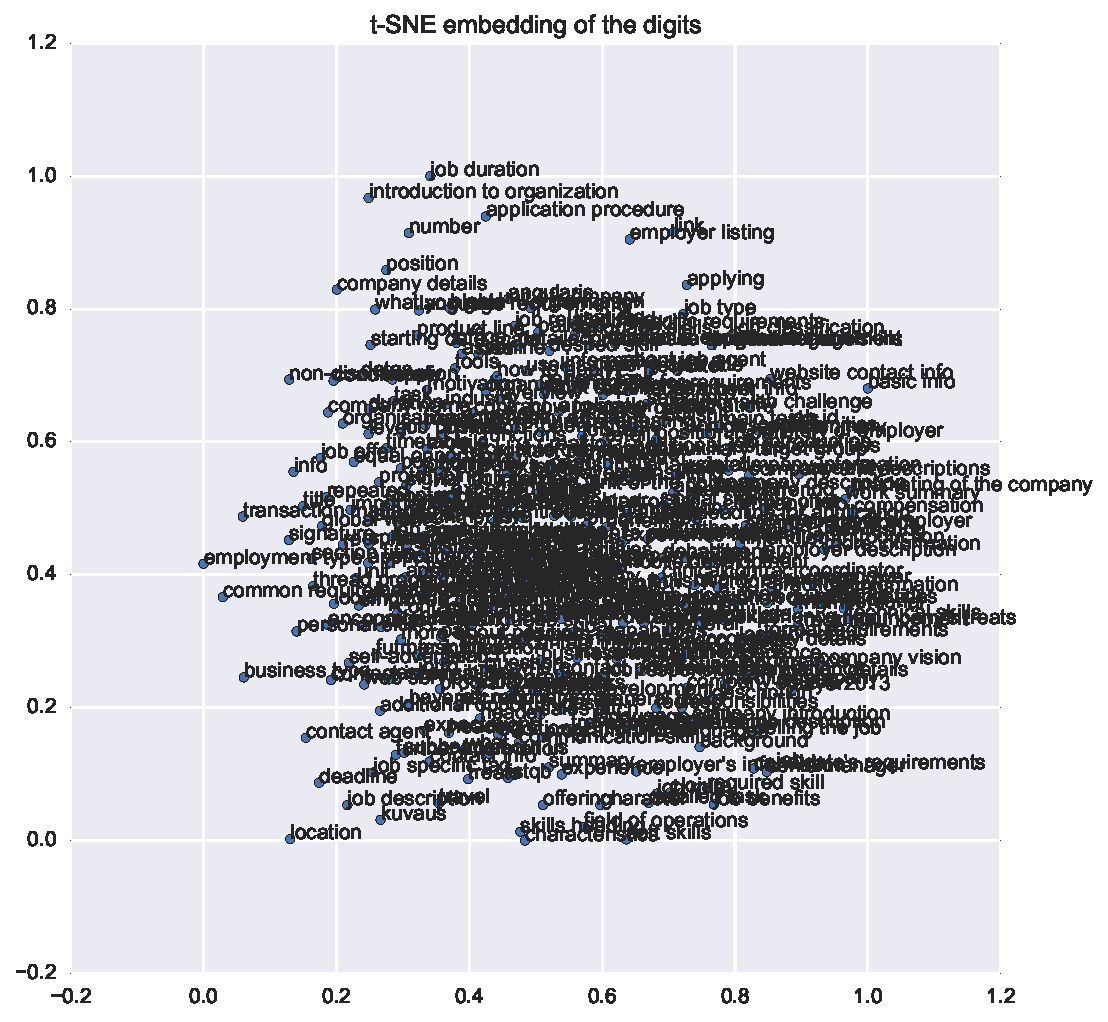
\includegraphics[width=\textwidth]{img/paragraph-data-tSNE.pdf}
    \caption{t-SNE Embedding}
\label{fig:paragraph-data-tSNE}
\end{figure}

\begin{figure}[h]
    \centering
    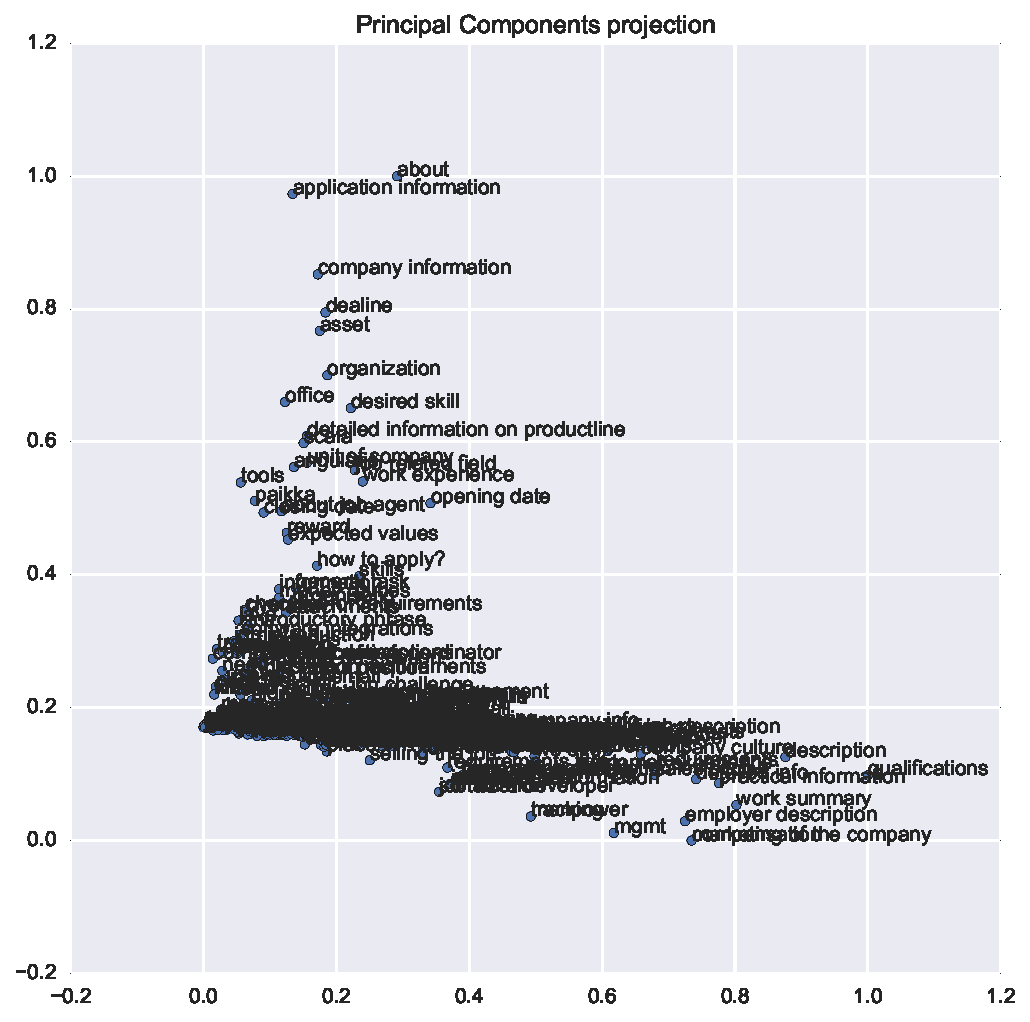
\includegraphics[width=\textwidth]{img/paragraph-data-principal-components-projection.pdf}
    \caption{Principal Components Projection}
\label{fig:paragraph-data-principal-components-projection}
\end{figure}

\todo{Comparison one-vs-rest and one-vs-one against linear machine}
\todo{Visualizations and embeddings of data in 2D (and decision boundaries?)}
\todo{show T-SNE embeddings of doc2vec vectors}



\subsubsection{Multi-class Sentence Classification}
\label{subs:Multi-class Sentence Classification}

% ----------- Data Sections



% ----------- Dataset2

\begin{figure}[h]
 % From http://localhost:8888/notebooks/thesis/experiments/vector-space-models/Vector%20Space%20Models.ipynb#Setup
    \centering
    \begin{subfigure}[b]{0.46\textwidth}
        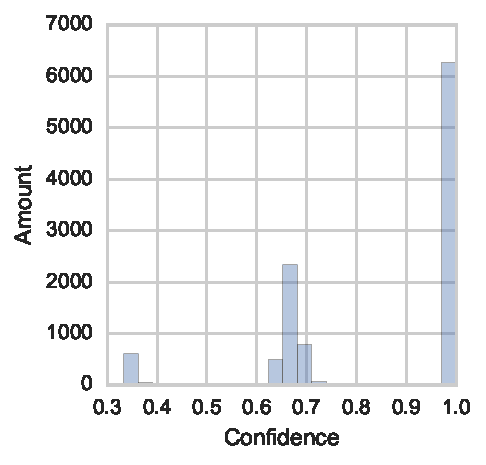
\includegraphics[width=\textwidth]{img/sentence-data-judgement-confidence.pdf}
        \caption{Confidence}
\label{fig:sentence-data-judgement-confidence}
    \end{subfigure}
~%add desired spacing between images, e. g. ~, \quad, \qquad, \hfill etc.
    %(or a blank line to force the subfigure onto a new line)
    \begin{subfigure}[b]{0.43\textwidth}
        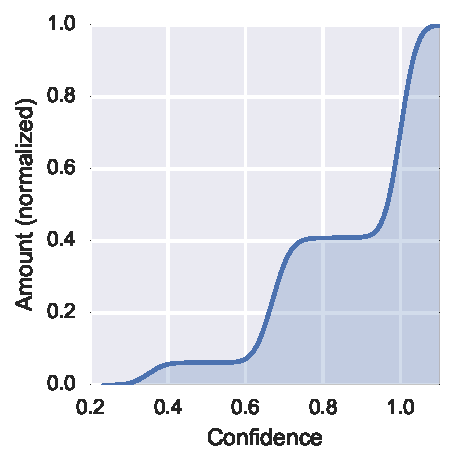
\includegraphics[width=\textwidth]{img/sentence-data-judgement-confidence-cumulative.pdf}
        \caption{Cumulative Confidence}
\label{fig:sentence-data-judgement-confidence-cumulative}
    \end{subfigure}
    \caption{Amount of label judgements versus label confidence of the sentence label data collected via crowdflower}
\label{fig:sentence-data-judgements}
\end{figure}
